% Do not change document class, margins, fonts, etc.
\documentclass[a4paper,oneside,bibliography=totoc]{scrbook}

% some useful packages (add more as needed)
\usepackage{scrhack}
\usepackage[utf8]{inputenc}
\usepackage{graphicx}
\usepackage{latexsym}
\usepackage{amsmath}
\usepackage{amssymb}
\usepackage{tabularx}
\usepackage{csquotes}
\usepackage{booktabs}
\usepackage{listings}
\usepackage{algorithm}
\counterwithin{algorithm}{chapter}
\usepackage{algorithmic}
\usepackage{csquotes}
\renewcommand{\algorithmiccomment}[1]{\hfill\textit{// #1}}
\usepackage[usenames,dvipsnames]{xcolor}
\usepackage[colorlinks,citecolor=Green]{hyperref}
\usepackage{lipsum}
\usepackage[printonlyused]{acronym}

% chicago citation style
\usepackage{natbib}
\bibliographystyle{chicagoa}
\setcitestyle{authoryear,round,semicolon,aysep={},yysep={,}} \let\cite\citep

% example enviroments (add more as needed)
\newtheorem{definition}{Definition} \newtheorem{proposition}{Proposition}

% Definition einer Turtle‑Sprache
\lstdefinelanguage{Turtle}{
  morekeywords={@prefix,@base,a},
  morekeywords=[2]{ex,exp,rdfs},
  morestring=[b]",
  morestring=[b]',
  sensitive=true,
  basicstyle=\small\ttfamily,
  keywordstyle=\color{blue},
  keywordstyle=[2]\color{magenta},
  commentstyle=\color{gray}\itshape,
  stringstyle=\color{OliveGreen},
  columns=fullflexible,
  breaklines=true,
  breakatwhitespace=false,
  literate={:}{{{\color{orange}:}}}1,
}

% Definition einer SPARQL‑Sprache
\lstdefinelanguage{SPARQL}{
  morekeywords={@prefix,@base,a,SELECT,WHERE},
  morekeywords=[2]{ex,exp,rdfs},
  morestring=[b]",
  morestring=[b]',
  sensitive=true,
  basicstyle=\small\ttfamily,
  keywordstyle=\color{blue},
  keywordstyle=[2]\color{magenta},
  commentstyle=\color{gray}\itshape,
  stringstyle=\color{OliveGreen},
  columns=fullflexible,
  breaklines=true,
  breakatwhitespace=false,
  literate={:}{{{\color{orange}:}}}1,
}

% Globales Styling für alle Listings
\lstset{
  language=Turtle,
  frame=single,
  numbers=left,
  numberstyle=\tiny\color{gray},
  numbersep=5pt,
  tabsize=2,
  captionpos=b,
  basicstyle=\small\ttfamily,
}

\begin{document}

\frontmatter
\subject{Master Thesis}
\title{Title of Your Master Thesis}
\author{Max Lautenbach\\
  (matriculation number XXXXXXXX)}
\date{\today}
\publishers{{\small Submitted to}\\
  Data and Web Science Group\\
  Dr.\ Sven Hertling\\
  University of Mannheim\\}
\maketitle

\chapter{Abstract}

% Your abstract goes here

\begingroup%
\hypersetup{hidelinks}%
\tableofcontents%
\endgroup

\chapter{List of Abbreviations}
\begin{acronym}
  \acro{RDF}{Resource Description Framework}
  \acro{URI}{Uniform Resource Identifier}
  \acro{RDFS}{Resource Description Framework Schema}
  \acro{OWL}{Web Ontology Language}
  \acro{SPARQL}{SPARQL Protocol and RDF Query Language}
  \acro{LM}{Language Model}
  \acro{LLM}{Large Language Model}
  \acro{ML}{Machine Learning}
\end{acronym}

\mainmatter

\chapter{Introduction}
\label{ch:intro}

% Your introduction goes here

\chapter{Background}
\label{ch:related_work}
In the following chapter, the necessary theoretical background to understand core concepts of this approach will be described. Therefore, the chapter will start with an explanation of knowledge graphs (section \ref{sec:knowledge_graphs}). Building on that foundation, a section on closed information extraction (section \ref{sec:closed_information_extraction}), which is the problem that is approached in this work, will follow. Afterwards the theoretical background on the multi-agent-system approach will be defined starting with the core language and embedding models (section \ref{sec:language_models} and \ref{sec:sentence_embeddings_vector_stores}) over to defining what AI agents and multi-agent-systems are (section \ref{sec:ai_agents} and \ref{sec:multi_agent_systems}), leading to a section on agent design best practises (section \ref{sec:agent_design}).
\section{Knowledge Graphs}
\label{sec:knowledge_graphs}
Knowledge graphs are a concept to store knowledge in a way that the semantic in the knowledge is machine-retrievable \cite{GomezPerez2017}. In order to accomplish this goal, knowledge graphs are directed graphs, whereas the nodes define real world entities and the edges define the relationsship between the entities \cite{Paulheim2016}. To define the domain and give a knowledge graph a set of rules, the types of entities and relations are predefined in what is called an ontology \cite{GomezPerez2017,Paulheim2016}. Following those definition, the ecosystem of knowledge graphs is build from three building blocks: knowledge graph construction, knowledge graph storage, knowledge graph consumption \cite{GomezPerez2017}.

Starting from the construction, knowledge graphs are represented in \ac{RDF}, which is the standard to represent knowledge graphs. \ac{RDF} is build of triples, whereas each triple could be seen as description of a relation by the three parts \textit{Start Node, Edge and Target Node}. All parts of the triple are either a resource identifier, a blank node or a literal. In the case of this work, the used resource identifier is a \ac{URI} like for example \textit{\url{http://example.org/entity/Angela_Merkel}}, that is why all chapters the term \ac{URI} will used consisent instead of change to more general or more specific identifiers. Exception to the general denotation by \acp{URI} are blank nodes and literals. Blank nodes is a concept where a resource could not be specified. This could be the case, if the relation that is described by the triple includes concepts like \textit{someone} or \textit{something}. Literals are simple values, like integers or strings \cite{VillazonTerrazas2017}.

The relation described by the triples can also be seen as a simple english sentence consisting of subject matching the start node, predicate matching the edge and object matching the target node. For each of those there are common rules, when defining the knowledge graph. Subjects can be either an \ac{URI} or a blank node. Predicates, which are called properties from now on as predicates are named properties throughout in knowledge graphs, can only be \acp{URI}. An Object can be an \ac{URI}, a blank node or a literal. Inheriting this concept the \ac{RDF} contains multiple syntactical representations of knowledge graphs, one of which Turtle is \cite{VillazonTerrazas2017}.

Turtle is build up of simple triple statements consisting of subject, property and object, where each part is separated by either a space, tabluation or whitespace. Each statement in turtle is terminated like a normal sentence using a dot. A \ac{URI} must be enclosed in angle brackets, whereas blank nodes can be represented with an underscore follow with a colon and an arbitrary name for the blank node instead of a \ac{URI} and Literals are enclosed in quote, where turtle interpreter either define the datatype of the value themselves or the datatype can be defined by the user. In the follow example, it can be seen how four sentences can be defined within the turtle format \cite{Tomaszuk2020}.


\begin{lstlisting}[language=Turtle, caption=Example of a Knowledge Graph in Turtle Format, label=lst:turtle_example, escapechar=@]
@\textcolor{gray}{\# Angela Merkel is member of the CDU.}@
<http://example.org/entity/Angela_Merkel> <http://example.org/property/member_of> <http://example.org/entity/CDU>.

@\textcolor{gray}{\# Angela Merkel is written "Angela Merkel".}@
<http://example.org/entity/Angela_Merkel> <http://www.w3.org/2000/01/rdf-schema#label> "Angela Merkel".

@\textcolor{gray}{\# Angela Merkel is greeted by someone.}@
<http://example.org/entity/Angela_Merkel> <http://example.org/property/greeted_by> _:b1.

@\textcolor{gray}{\# This someone works for Friedrich Merz.}@
_:b1 <http://example.org/property/works_for> <http://example.org/entity/Friedrich_Merz>.
\end{lstlisting}

In order to simplify the turtle statements, prefixes can be defined. Those prefixes corralate to a namespace, which is a path in the \ac{URI} which multiple resource are stored under. A prefix is defined using \textit{@prefix}, the name of the prefix followed by a colon (i.e. \textit{ex:}) and the namespace itself. In the shown example using prefixes could simplify the turtle statements to the following \cite{Tomaszuk2020}:

\begin{lstlisting}[language=Turtle, caption=Example of a Knowledge Graph in Turtle Format, label=lst:turtle_example]
@prefix ex: <http://example.org/entity/>
@prefix exp: <http://example.org/property/>
@prefix rdfs: <http://www.w3.org/2000/01/rdf-schema#>

ex:Angela_Merkel exp:member_of ex:CDU.
ex:Angela_Merkel rdfs:label "Angela Merkel".
ex:Angela_Merkel exp:greeted_by _:b1.
_:b1 exp:works_for ex:Friedrich_Merz.
\end{lstlisting}

Besides defining the entities and their relationship, turtle is also used to implement ontologies. In general ontologies can be defined using \ac{RDFS} or \ac{OWL}, which itself is an extension to \ac{RDFS}. The idea behind \ac{RDFS} is to provide a standardised way to define classes and properties for a knowledge graph. In addition, \ac{RDFS} can make the semantic of a knowledge graph more extensive by providing restrictions or indents on a class. One apparent restrictions is the domains and ranges attached on properties. Domains and ranges are type restrictions on the subject (domain) and object (range) of a triple. When there is a property like \textit{exp:member\_of} is defined, the ontology can hold the domain \textit{ex:human} and the range \textit{ex:organisation}, which means the every subject \textit{S} that is member of an object \textit{O} must be of type \textit{ex:human}, whereas the object must be of type \textit{ex:organisation}. As \ac{RDFS} is limited in experessive power, \ac{OWL} was developed as extension providing ideas like symmetric properties like \textit{exp:married\_to}, which when A is married to B, we can imply that B is married to A. \ac{OWL} also provides an extensive set of possible restrictions, which opens the opportunity to design complex restrictions on either classes or properties \cite{VillazonTerrazas2017}.

Following up to the building block of knowledge graph construction, it is necessary to introduce triple stores as the building block of knowledge graph storage. Triple stores are build to save and retrieve identities form a triplex collection, which means that triple stores are connection construction and retrieval. The triplex collection has to comply with the \ac{RDF} standard \cite{Rusher2003}. One triple store implementation is Apache Jena. Jena provides a whole triple store stack, allowing to manipulate and retrieve an \ac{RDF} graph via API or direct I/O modules in Java. In addition, Jena supports all mentioned standard like \ac{RDF}, \ac{RDFS} and \ac{OWL} \cite{Carroll2004}. To support the de-facto standard knowledge graph query language \ac{SPARQL} \cite{VillazonTerrazas2017}, the Apache Jena Toolset implements Jena Fuseki which is working as a \ac{SPARQL} server \cite{Chokshi2022}.

The idea of \ac{SPARQL} is to retrieve data from a \ac{RDF} knowledge graph, but also to manipulate data in it. The language is following the standards of turtle, when it comes to query construction. Three most essential query types are select, ask and insert queries. Select queries are able to retrieve content from the graph. Ask queries are simplified select queries, that can just acknowledge on an existance of the requested query. Insert queries are ones to manipulate the data in the graph \cite{VillazonTerrazas2017}.

In general a \ac{SPARQL} query begins with the query type followed with the \textit{WHERE} keyword and the query definition. In the case of select queries, the query type keyword is followed by variables, which are defined be a leading question mark followed by the variable name (i.e. \textit{?organisation}). As \ac{SPARQL} follows the turtle language also prefixes can be defined. In addition \ac{SPARQL} queries can take filtering and query options like limits or offsets \cite{VillazonTerrazas2017}. To show an example, if you want to search the organisations Angela Merkel is member of, a \ac{SPARQL} query could look like this:

\begin{lstlisting}[language=SPARQL, caption=Example of a SPARQL Query, label=lst:turtle_example]
  @prefix ex: <http://example.org/entity/>
  @prefix exp: <http://example.org/property/>
  
  SELECT ?organisation WHERE {
    ex:Angela_Merkel exp:member_of ?organisation
  }
  \end{lstlisting}

As all building blocks of a knowledge graphs are declared, the goal is now to introduce one use case of knowledge graphs to show the capabilities but also challenges in leveraging knowledge graphs in real world use cases. A project named HAVAS 18 aimed to monitor start-up activities, tech trends and tech talents leveraging knowledge graphs. This comes by leveraging existing relationships between the mentioned entities on social networks. This could reveal relevant relations and create a better understanding how start-ups, tech trends and tech talents arise and evolve. As social networks can already provide structured relationship data, the data basis of the knowledge graph can be extracted \cite{Monti2017}. On the other side \citep{Monti2017} states, that the main challenges of this project were entity resolution and disambiguation as well as the processing of unstructured data. This already shows up challenges, that this work tries to solve.

In addition to such specific use cases, there are approaches, which try to represent the largest online encyclopoedia Wikipedia into a knowledge graph. Two present approaches are Wikidata and DBpedia. The goal of Wikidata was to establish a knowledge management for factual information in Wikipedia. Leveraging knowledge graph technology the idea was to eliminate redundancies and create multi-language support. Therefore, Wikidata is also a community-based project, where the community can make changes in the graph. In addition, Wikidata is nowadays the factual information knowledge store integrated into Wikipedia \cite{Vrandecic2014}. In addition, DBpedia is another knowledge graph employed to provide data for semantic web applications. Other than in Wikidata, DBpedia use extraction frameworks leveraging syntactical structured constructs from MediaWiki to convert Wikipedia dumps to \ac{RDF}.

As a conclusion, knowledge graphs can provide semantically rich data, by leveraging the graph data structure together with standardised frameworks and languages build around the knowledge graph concept. In addition, knowledge graphs are publically available in immense size and are open to use. Nevertheless, when developing use cases utilising knowledge graphs, the challenges could come down to process unstructured data and detect ambiguated entities.

\section{Closed Information Extraction}
\label{sec:closed_information_extraction}
Closed information extraction is the problem area of extracting triples out of an unstructured text, whereas each part of triple must match the underlying knowledge graph \cite{Josifoski2021}. This means that the extracted entities and properties have to match the exact string, that can be mapped into the knowledge graph. This differs from open information extraction, as there the textual information gets convert in free-form triples \cite{Etzioni2008}.
Another concept in the area of information extraction is relation extraction, which is focussed on identifying the relation between entities, which also includes detecting entities \cite{Zhao2024}. Relation extraction differs from open relation extraction, as the type and structure of relations are already defined \cite{Kamp2023}. All problems are sub-problems of the field of information extraction, which is defined as the general process to extract entities and relations out of a text \cite{Etzioni2008}.

As especially relation extraction and closed information extraction share many similarities, the challenges and solutions are also similar. The first challenge is about to identify and extract entities out of a text. From there on, entities can be already linked to a knowledge graph in the case of closed information extraction. In this case entity extraction necessarily means also entity disambiguation, as there might be entities using the same name in the knowledge graph. Using the identified entities, relations must be detected between them and those relations have to be classified. Afterwards a mapping of those relations into the knowledge graph must be done when processing a closed information extraction task \cite{Josifoski2021,Zhao2024}.

To process those tasks, there are two approaches: A pipeline or a joint-approach. The pipeline approaches work through those tasks step-by-step. In some cases the exact steps are variied as tasks can be splited up or joined. In joint approaches all steps happen at the same time but implicitly. This is an approach to reduce error propagation throughout the single steps in the pipelines by combining them, in order to optimised methods towards the overall target of producing correct triples \cite{Zhao2024,Josifoski2021}.

Whereas the ideas of all subproblems of information extraction remains the same, \citep{Josifoski2021} states, that especially open information extraction techniques are not applicable to closed information extraction. This is grounded in the complexity of closed information extraction, being constraint to a knowledge base. Therefore, closed information extraction requires structured output that is ready to be mapped onto entities and properties in a knowledge graph \cite{Josifoski2021}.

Overall closed information extraction is a very restricted subclass of information extraction where the additional challenge of mapping entities and properties to a knowledge base is added to the remaining challenges. Those challenges are covering entity extraction, disambiguation and linking together with the actual relation extraction and linking. Each of this steps can produce errors, which is why either pipeline approaches are used, where each step is tried to be as error-resistant as possible or joint approaches are used, which can be optimised towards the overall goal.

\section{Language Models}
\label{sec:language_models}
A \ac{LM} is a \ac{ML} model, that at its core is able to predict the probabilities of how a text is going to be completed based on the previous text\cite{Radford2019}. Since the original publication by \citep{Vaswani2023} most present \acp{LM} are build out of two components, the tokenizer and the transformel model. The tokenizer transforms parts of a text into a integers. Therefore, the integers are like a index in a vocabulary mapping a character sequence to an integer \cite{Sennrich2016}. In present models like the GPT-models the existing tokenizer is a byte-pair encoding \cite{Radford2019}. This byte-pair encoding works by intialising a vocabulary using single characters. Afterwards frequent character sequences will be merged iteratively, create new tokens. This will be done until a defined maximum number of tokens in the vocabulary is reached \cite{Sennrich2016}. With that explained, a \ac{LM} can be mathematically formulated as a conditional probability $P$ of the token $t_i$ under the condition of all previous tokens:
\begin{equation}
  P(t_i|t_1,...,t_{i-1}).
\end{equation}

The core part of a \ac{LM} is the transformer. Transformers itself are \ac{ML} models that concept of Multi-Head-Attention Layers and Feed-Fordward Layers. Attention is a concept to encode previously tokens ($t_1,...,t_{i-1}$) and their relation to the current token $t_i$ into the encoded representation of the current token. The implementation of this concepts requires an learned embedidng of all tokens and three learnable weight matrices. An embedding is in this case a trained mathematical representation of a token. The weight matrices split up in one weight matrix $W^Q$ for the current token and two weight matrices $W^K, W^V$ for the previous tokens \cite{Vaswani2023}. The idea behind this concept is, that those weight matrices are able to detect relations like adjectives and therefore influence the encoding of a token \cite{Sanderson2024}. For instance, when the text \enquote{... the former german chancelor Angela Merkel ...} is processed by the attention layer, the attention mechanism could encode \enquote{former german} into the token of \enquote{chancelor}. It has to be mentioned, that this is an example and the exact behavior of the attention layer could differ \cite{Sanderson2024}.

Following this idea, \citep{Vaswani2023} proposed the concept of multi-head attention to learn multiple weight matrices and run the matrix multiplication done by the attention mechanism multiple times in parallel. Afterwards the result of all attention heads are concatenated and projected using the Softmax function \cite{Vaswani2023}. Therefore, multi-head attention could also be able to identify various kinds of relationships inside a sentence \cite{Sanderson2024}. In addition to multi-head attention, a position encoding is inserted into the embeddings of the tokens \cite{Vaswani2023}. In addition, each output of the attention respective the feed forward layer gets added to the initial input to this layer and afterwards get normalized. The Transformer is completed by a linear layer mapping the vector representation back on the vocabulary and a softmax layer to get a probability distribution across the vocabulary \cite{Vaswani2023}. Figure \ref{fig:transformer} shows the overall composition of transformers with the encoder component on the left and the decoder component on the right. As following explanations focusses on the already explained components the masked-multi-head-attention and encoder-decoder split will not be covered.

\begin{figure}[h]
  \centering
  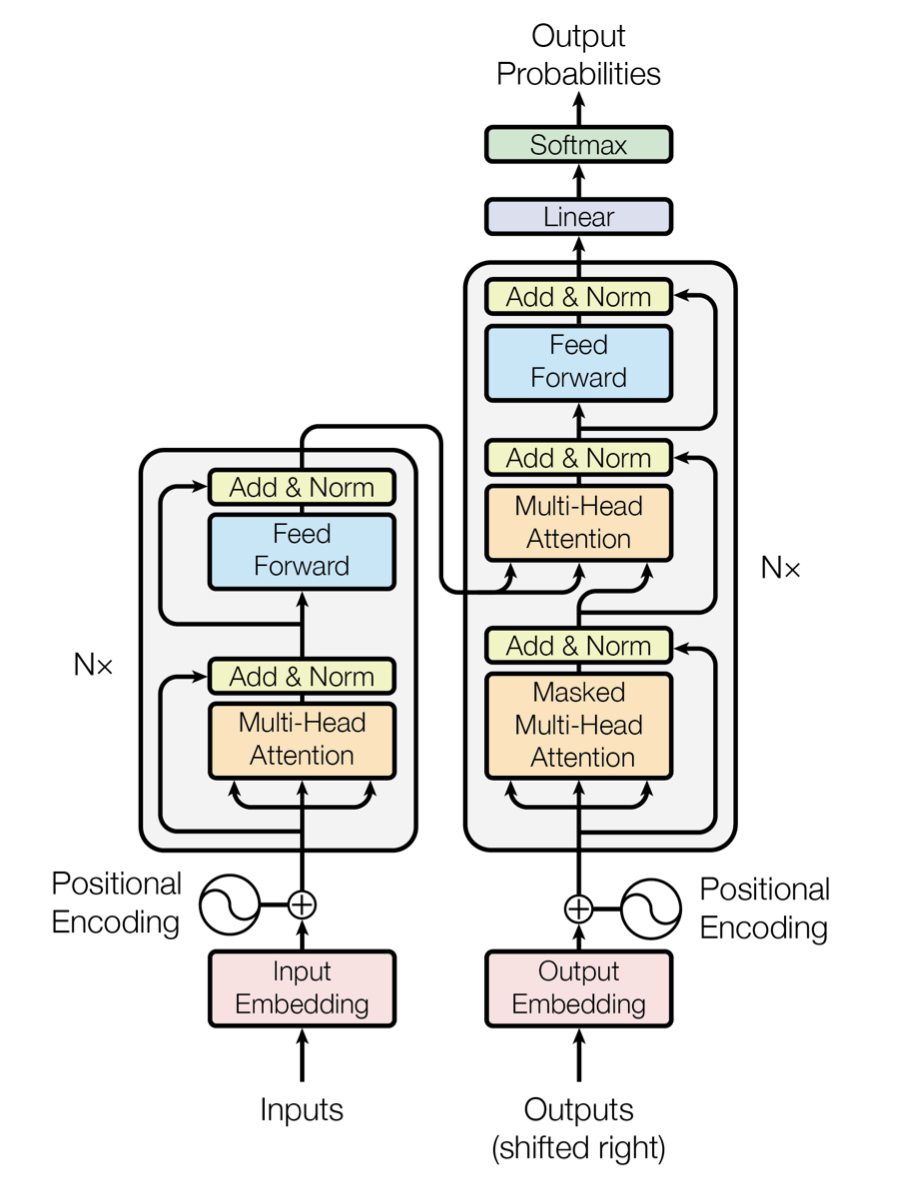
\includegraphics[width=0.5\textwidth]{figures/Transformer.png}
  \caption{Architecture of a Transformer model. \cite{Vaswani2023}}
  \label{fig:transformer}
\end{figure}

\begin{itemize}
  \item What are LLMs?
  \item How do they work?
  \item What capabilities do they have?
  \item Softmax Temperature and Seeds
\end{itemize}
\section{Sentence Embeddings and Vector Stores}
\label{sec:sentence_embeddings_vector_stores}
\section{AI Agents}
\label{sec:ai_agents}
\begin{itemize}
  \item What is an Agent
  \item What is an AI Agent
  \item How are Tools incorporated
  \item Which Frameworks do exist
\end{itemize}
\section{Multi-Agent-Systems}
\label{sec:multi_agent_systems}
\begin{itemize}
  \item What are Multi-Agent Systems
  \item What Architectures exist for MAS
\end{itemize}
\section{Agent Design}
\label{sec:agent_design}
\begin{itemize}
  \item Building effective agents \cite{Anthropic2024}
  \item Prompt Engineering \cite{Schulhoff2025}
\end{itemize}

\chapter{Related Work}
\label{ch:related_work_chapter}
\begin{itemize}
  \item What Models or Work do exists in the cIE and MAS Context?
  \item What Dataset do exist in the cIE Context? How are they compared? How are they extracted?
  \item GenIE \cite{Josifoski2021}
  \item synthIE (Model and Dataset) \cite{Josifoski2023}
  \item REBEL (Model and Dataset) \cite{HuguetCabot2021}
  \item DISCIE \cite{Moeller2024}
  \item AgentRE \cite{Shi2024}
\end{itemize}

% Your literature review goes here

\chapter{Approach}
\label{ch:approach}
\section{Agent Architectures}
\label{sec:agent_architectures}
\subsection{Baseline}
\label{subsec:baseline}
\subsection{Supervisor}
\label{subsec:supervisor}
\subsection{ReAct}
\label{subsec:react}
\subsection{Network}
\label{subsec:network}

\section{Agent Tools}
\label{sec:agent_tools}
\subsection{URI Search}
\label{subsec:uri_search}
\subsection{Network Traversal}
\label{subsec:network_traversal}
\subsection{Message Deletion}
\label{subsec:message_deletion}
\subsection{Semantic Validation}
\label{subsec:semantic_validation}
\subsection{Turtle to Label}
\label{subsec:turtle_to_label}
\section{Evaluation Setup}
\label{sec:evaluation_setup}
\subsection{Dataset}
\label{sec:dataset}
\begin{itemize}
  \item synthIE
\end{itemize}
\subsection{Wikidata}
\label{sec:wikidata}
\begin{itemize}
  \item How does Wikidata looks like?
\end{itemize}
\begin{itemize}
  \item Langgraph
  \item 2 Datasplits on synthIE Text (Train Val, Test)
  \item 2 Datasplits on synthIE Code (Train , Test) (optional)
  \item Results on 5/50 Examples
  \item Cerebras, SambaNova Cloud, vLLM on 2x A100
  \item Models: Llama 3.3 70B (Mainly), Tests with o3-mini, Llama 4 ...
\end{itemize}
% Your first main chapter goes here

\chapter{Evaluation}
\label{ch:evaluation}
\section{Evaluation Metrics}
\label{sec:evaluation_metrics}
\begin{itemize}
  \item Definition Positive/Negative Triple \cite{Josifoski2021}
  \item F1-Score, Precision, Recall
  \item With Parents, With Related
\end{itemize}


\section{Evaluation Configurations}
\label{sec:evaluation_configurations}
\subsection{Initial Baseline Setup}
\label{subsec:initial_baseline_setup}
\begin{itemize}
  \item Supervisor Agent
  \item Entity Extractor
  \item Relation Extractor
  \item URI Retrieval Agent
\end{itemize}

\subsection{Modularization of Agent Tasks}
\label{subsec:modularization_agent_tasks}
\begin{itemize}
  \item Decomposition of the Supervisor Agent into:
        \begin{itemize}
          \item Planner
          \item Agent Instructor
          \item Result Checker
          \item Result Formatter
        \end{itemize}

  \item Introduction of URI-Search Filters (On Label OR Description)
\end{itemize}

\subsection{Error Message Incorporation}
\label{subsec:error_message_incorporation}
\begin{itemize}
  \item Integration of error messages
  \item Improved state monitoring and feedback
  \item Predicate Extractor in Gen1
  \item Baseline extended with URI Response Summary
\end{itemize}

\subsection{Task Simplification and State Refinement}
\label{subsec:task_simplification_state_refinement}
\begin{itemize}
  \item Simplification of agent state representations (e.g., Gen1 → Gen1v2)
\end{itemize}

\subsection{One-Agent Architecture with Tool Usage}
\label{subsec:one_agent_architecture_tool_usage}
\begin{itemize}
  \item Centralization of all tasks into a single agent
  \item Use of external tools to perform sub-tasks
\end{itemize}

\subsection{URI Retrieval Filtering}
\label{subsec:uri_retrieval_filtering}
\begin{itemize}
  \item Switch to Filtering on Entities and Properties
\end{itemize}

\subsection{Knowledge Graph Integration}
\label{subsec:knowledge_graph_integration}
\begin{itemize}
  \item Incorporation of domain-specific knowledge via:
        \begin{itemize}
          \item Network Traversal (and why deleted later)

        \end{itemize}
\end{itemize}

\subsection{Full Network Agent Architecture}
\label{subsec:full_network_agent_architecture}
\begin{itemize}
  \item Combination of insights from Baseline, Gen1, and One-Agent approaches
  \item Network-based collaboration between specialized agents
  \item Dynamic use of tools and agent interactions
  \item Few-Shot Prompting
  \item Update URI Search Modes
  \item Semantic Validation
  \item Turtle to Label conversion
\end{itemize}

\subsection{Performance Increases of Gen2 to One Agent and Baseline Architecture}
\label{subsec:performance_increases_gen2}
\begin{itemize}
  \item One Agent
  \item Baseline
\end{itemize}

\subsection{LLM Model Variation}
\label{subsec:llm_model_variation}
\begin{itemize}
  \item Various models at various stages and show results
  \item Elaborate on why to choose Llama 3.3 70B over other models
\end{itemize}

\section{Discussion}
\label{sec:discussion}


\chapter{Conclusion and Outlook}
\label{ch:conclusion_outlook}

% Your conclusions go here

\bibliography{references/references}

\appendix
\chapter{Additional Material}
\label{ch:additional_material}

% Your additional material goes here

\backmatter
\chapter{Ehrenwörtliche Erklärung}
\label{ch:declaration}

Ich versichere, dass ich die beiliegende Bachelor-, Master-, Seminar-, oder
Projektarbeit ohne Hilfe Dritter und ohne Benutzung anderer als der angegebenen
Quellen und in der untenstehenden Tabelle angegebenen Hilfsmittel angefertigt
und die den benutzten Quellen wörtlich oder inhaltlich entnommenen Stellen als
solche kenntlich gemacht habe. Diese Arbeit hat in gleicher oder ähnlicher Form
noch keiner Prüfungsbehörde vorgelegen. Ich bin mir bewusst, dass eine falsche
Erklärung rechtliche Folgen haben wird.

\begin{center}
  \textbf{Declaration of Used AI Tools} \\[.3em]
  \begin{tabularx}{\textwidth}{lXlc}
    \toprule
    Tool & Purpose & Where? & Useful? \\
    \midrule
    % Add your AI tools here
    \bottomrule
  \end{tabularx}
\end{center}

\vspace{2cm}
\noindent Unterschrift\\
\noindent Mannheim, den XX.~XXXX 2024 \hfill

\end{document}
